\documentclass[11pt,a4paper]{article}
\UseRawInputEncoding
\usepackage[utf8]{inputenc}
\usepackage[T1]{fontenc}
\usepackage{graphicx}
\usepackage{amsmath}
\usepackage{amssymb}
\usepackage{hyperref}
\usepackage{geometry}
\geometry{a4paper, margin=1in}
\usepackage{listings}
\usepackage{pgf}
\usepackage{tikz}
\title{\textbf{Analyse des certificats SSL/TLS et des vulnérabilités des clés RSA}}
\author{	\textbf{Daoudi Amir Salah Eddine, Heloui Youssef, Baye Diop Cheikh} \\
Module : Cryptographie Appliquée}
\date{\today}

\begin{document}

\maketitle

\begin{abstract}
Dans un contexte où les cyberattaques se multiplient, cette analyse contribue à renforcer les fondations des communications sécurisées en identifiant des faiblesses exploitables dans les certificats SSL/TLS.
Ce rapport présente une analyse approfondie des certificats SSL/TLS, en mettant l'accent sur la distribution des tailles de clés RSA, la détection des doublons, et les vulnérabilités liées aux facteurs communs identifiés par le calcul des PGCD. Le pipeline mis en place inclut l'acquisition asynchrone des certificats, leur tri par taille, et l'exécution d'analyses automatisées pour identifier les risques potentiels. Les scripts et données utilisés pour ce projet sont accessibles via les dépôts suivants :
\begin{itemize}
    \item GitHub : \url{https://github.com/DaoudiAmir/SSL-TLS}
    \item GitLab : \url{https://gitlab.esiea.fr/helouiyoussef/crypto}
\end{itemize}
Ce projet a été réalisé dans le cadre du module de Cryptographie Appliquée pour la classe TD48.
\end{abstract}


\tableofcontents

\section{Introduction}
Les certificats SSL/TLS jouent un rôle crucial dans la sécurisation des communications sur Internet en garantissant l'authenticité et la confidentialité des échanges. Cependant, l'efficacité de ces mécanismes dépend fortement de la solidité des clés cryptographiques utilisées, notamment celles générées par l'algorithme RSA. Les vulnérabilités liées à une mauvaise gestion des clés, telles que l'utilisation de facteurs communs ou la réutilisation des modules, peuvent sérieusement compromettre la sécurité des systèmes.

Dans ce contexte, ce projet vise à analyser une grande base de certificats SSL/TLS pour détecter d'éventuelles failles cryptographiques, en se concentrant sur les points suivants :
\begin{itemize}
    \item La distribution des tailles de clés RSA dans les certificats collectés.
    \item L'identification de doublons parmi les clés RSA.
    \item La détection de vulnérabilités liées à des facteurs communs dans les modules RSA à travers le calcul des PGCD (Plus Grand Commun Diviseur).
\end{itemize}

Ce travail s'appuie sur une méthodologie structurée, allant de l'acquisition asynchrone des certificats à leur analyse détaillée à l'aide de scripts Python spécialisés. Le pipeline mis en place comprend plusieurs étapes clés, notamment :
\begin{enumerate}
    \item L'acquisition massive de certificats depuis des sources publiques comme \texttt{crt.sh}.
    \item Le tri et la classification des certificats par taille de clé.
    \item La conversion des données en formats analytiques tels que CSV.
    \item L'analyse avancée des données pour détecter des problèmes structurels ou des failles de sécurité.
\end{enumerate}

Les résultats obtenus permettront d'illustrer les pratiques actuelles en matière de gestion des certificats et des clés RSA, et de proposer des recommandations pour renforcer la sécurité des infrastructures cryptographiques.

\section{Organisation du code et structure}

Pour garantir une analyse efficace et modulaire, le projet a été organisé selon une structure bien définie, avec des répertoires dédiés à l'acquisition des certificats, à leur traitement, et aux résultats générés. Cette organisation facilite également la maintenance et l'extension future du pipeline. Voici une description détaillée de la structure :

\subsection{Structure des répertoires}
Le projet est divisé en plusieurs répertoires principaux, chacun ayant un rôle spécifique dans le pipeline. Voici un aperçu de cette structure :
\begin{lstlisting}[basicstyle=\small]
.
├── CertificateAcquisition/
│   ├── AsyncDownload.py      # High-performance certificate downloader
│   ├── NewProxyList.py       # Dynamic proxy management system
│   ├── TestAllProxyList.py   # Automated proxy validation
│   ├── getNewProxyList.py    # Proxy list updater
│   └── Requirements.txt      # Acquisition module dependencies
│
├── CertificateAnalysis/
│   ├── CERT by Size/         # Organized certificate storage
│   ├── DUPES/               # Duplicate certificates storage
│   ├── GCD/                 # GCD analysis results
│   ├── CSV/                 # Certificate data in CSV format
│   ├── RemoveNotRSA.py       # Certificate type filter
│   ├── Sort.py              # Multi-threaded certificate sorter
│   ├── certtocsv.py         # Data conversion utility
│   ├── findDupes.py         # Duplicate detection system
│   ├── findGCD.py           # Cryptographic analysis tool
│   ├── run_analysis_only.sh # Standalone analysis script
│   └── Requirements.txt     # Analysis module dependencies
│
└── projectGUI.sh            # Interactive control interface

\end{lstlisting}

\subsection{Description des modules principaux}
Chaque répertoire et script joue un rôle spécifique dans le pipeline. Voici une explication détaillée de chaque composant :

\paragraph{Répertoire Acquisition/}
Ce répertoire contient les scripts dédiés à l'acquisition des certificats depuis des sources publiques. Les principaux scripts incluent :
\begin{itemize}
    \item \texttt{AsyncDownload.py} : Télécharge les certificats en masse de manière asynchrone depuis \texttt{crt.sh}, en utilisant des requêtes parallèles pour améliorer la vitesse.
    \item \texttt{getNewProxyList.py} : Récupère des listes de proxys publics pour contourner les limitations imposées par les serveurs.
    \item \texttt{TestAllProxyList.py} : Vérifie la validité et la disponibilité des proxys, générant une liste optimisée pour le pipeline.
    \item \texttt{NewProxyList.py} : Contient une liste de proxys valides, utilisée par \texttt{AsyncDownload.py}.
\end{itemize}

\paragraph{Répertoire Analysis/}
Ce répertoire regroupe les scripts responsables du traitement et de l'analyse des certificats téléchargés :
\begin{itemize}
    \item \texttt{Sort.py} : Trie les certificats en fonction de la taille de leur clé RSA et les organise dans des répertoires correspondants.
    \item \texttt{RemoveNotRSA.py} : Filtre et supprime les certificats qui n'utilisent pas l'algorithme RSA.
    \item \texttt{certtocsv.py} : Convertit les certificats en format CSV, en extrayant des informations clés telles que le module et l'exposant.
    \item \texttt{findDupes.py} : Identifie les certificats partageant des modules identiques, signalant ainsi des doublons.
    \item \texttt{findGCD.py} : Analyse les modules des clés pour détecter des facteurs communs entre plusieurs certificats.
    \item \texttt{run_analysis_only.sh} : Un script bash qui automatise l'exécution des étapes d'analyse dans un ordre prédéfini.
\end{itemize}

\paragraph{Répertoires CERT, CERT by Size, DUPES et GCD}
\begin{itemize}
    \item \texttt{CERT/} : Contient les certificats bruts téléchargés.
    \item \texttt{CERT by Size/} : Répertoire de certificats triés par taille de clé (1024 bits, 2048 bits, etc.).
    \item \texttt{DUPES/} : Fichiers CSV répertoriant les doublons détectés parmi les certificats.
    \item \texttt{GCD/} : Résultats des analyses de PGCD, identifiant les modules ayant des facteurs communs.
\end{itemize}

\section{Pipeline d'analyse des certificats}

Le pipeline mis en place pour ce projet repose sur une série d'étapes interconnectées qui permettent de traiter efficacement un grand volume de certificats SSL/TLS. Cette section décrit chaque étape en détail.

\subsection{Schéma du pipeline}
Le pipeline est structuré comme suit :
\begin{figure}[h!]
    \centering
    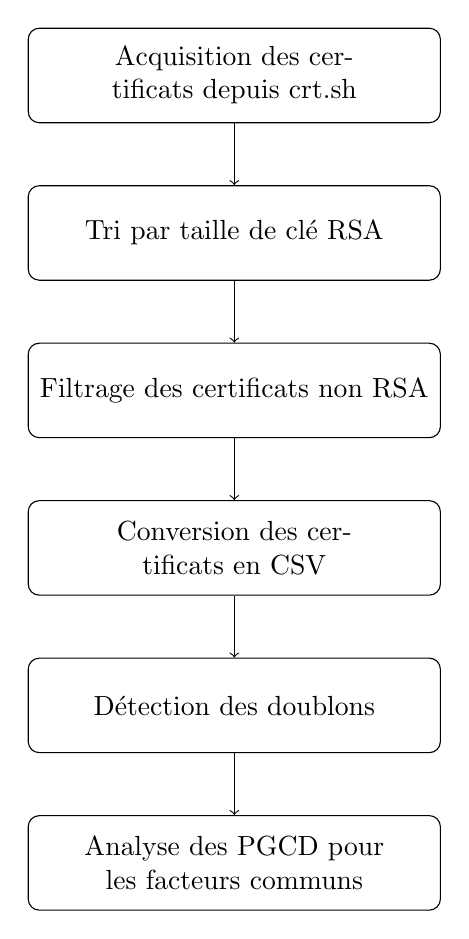
\begin{tikzpicture}[node distance=2cm, auto]
        \node (start) [rectangle, draw, text width=5cm, text centered, rounded corners, minimum height=1.2cm] {Acquisition des certificats depuis crt.sh};
        \node (sort) [rectangle, draw, below of=start, text width=5cm, text centered, rounded corners, minimum height=1.2cm] {Tri par taille de clé RSA};
        \node (filter) [rectangle, draw, below of=sort, text width=5cm, text centered, rounded corners, minimum height=1.2cm] {Filtrage des certificats non RSA};
        \node (convert) [rectangle, draw, below of=filter, text width=5cm, text centered, rounded corners, minimum height=1.2cm] {Conversion des certificats en CSV};
        \node (duplicates) [rectangle, draw, below of=convert, text width=5cm, text centered, rounded corners, minimum height=1.2cm] {Détection des doublons};
        \node (gcd) [rectangle, draw, below of=duplicates, text width=5cm, text centered, rounded corners, minimum height=1.2cm] {Analyse des PGCD pour les facteurs communs};
        
        \draw[->] (start) -- (sort);
        \draw[->] (sort) -- (filter);
        \draw[->] (filter) -- (convert);
        \draw[->] (convert) -- (duplicates);
        \draw[->] (duplicates) -- (gcd);
    \end{tikzpicture}
    \caption{Schéma du pipeline d'analyse des certificats.}
\end{figure}

\subsection{Description détaillée des étapes}

\paragraph{1. Acquisition des certificats}
L'étape initiale consiste à collecter un grand nombre de certificats SSL/TLS depuis des sources publiques comme \texttt{crt.sh}. Pour maximiser l'efficacité et contourner les limitations imposées par le serveur, les scripts suivants sont utilisés :
\begin{itemize}
    \item \texttt{AsyncDownload.py} : Ce script envoie des requêtes HTTP asynchrones pour télécharger les certificats en parallèle. Il exploite la bibliothèque Python \texttt{asyncio} pour gérer efficacement des milliers de connexions.
    \item \texttt{getNewProxyList.py} et \texttt{TestAllProxyList.py} : Ces scripts fournissent et valident des proxys pour éviter les blocages liés aux limitations de requêtes.
\end{itemize}

\paragraph{2. Tri par taille de clé RSA}
Une fois les certificats téléchargés, ils sont triés en fonction de la taille de leur clé RSA. Cette étape est réalisée à l'aide de \texttt{Sort.py}, qui extrait la taille de chaque clé publique et déplace les fichiers dans des répertoires spécifiques, tels que \texttt{./CERT by Size/1024/}.

\paragraph{3. Filtrage des certificats non RSA}
Tous les certificats qui n'utilisent pas l'algorithme RSA sont exclus du pipeline. Le script \texttt{RemoveNotRSA.py} valide chaque certificat en s'assurant que la clé publique est de type \texttt{RSAPublicKey}, et supprime les certificats invalides.

\paragraph{4. Conversion des certificats en format CSV}
Pour simplifier les étapes suivantes, les certificats sont convertis en fichiers CSV à l'aide de \texttt{certtocsv.py}. Les informations extraites incluent :
\begin{itemize}
    \item L'identifiant unique du certificat.
    \item Le module (\texttt{modulus}) de la clé publique.
    \item L'exposant (\texttt{exponent}) de la clé publique.
\end{itemize}

\paragraph{5. Détection des doublons}
Le script \texttt{findDupes.py} identifie les certificats partageant des modules identiques. Ces doublons peuvent indiquer des erreurs dans la génération des clés ou une mauvaise gestion des certificats.

\paragraph{6. Analyse des PGCD pour les facteurs communs}
L'étape finale consiste à rechercher des facteurs communs entre les modules de différentes clés RSA. En cas de partage d'un facteur commun, la clé peut être compromise. Cette analyse est réalisée par \texttt{findGCD.py}, qui utilise un algorithme optimisé de calcul des PGCD.

\subsection{Avantages du pipeline}
Ce pipeline offre plusieurs avantages clés :
\begin{itemize}
    \item \textbf{Scalabilité} : La collecte et l'analyse peuvent être effectuées sur des millions de certificats grâce à l'utilisation de processus parallèles.
    \item \textbf{Reproductibilité} : Les scripts permettent une exécution automatisée et cohérente.
    \item \textbf{Modularité} : Chaque étape peut être mise à jour ou remplacée sans affecter les autres composants.
\end{itemize}

\\section{Résultats}

Cette section présente les résultats obtenus à chaque étape du pipeline, mettant en lumière les observations clés sur les certificats analysés.

\subsection{Distribution des tailles de clés RSA}
Les certificats analysés ont été classés par taille de clé, révélant une distribution principalement concentrée autour de certaines tailles standard : 1024, 2048, et 4096 bits. Ces tailles sont conformes aux pratiques courantes dans l'industrie, mais elles reflètent également une tendance à adopter des tailles plus grandes pour des raisons de sécurité.

Exemple de distribution observée :
\begin{lstlisting}[language=Python, basicstyle=\small]
1024 bits: 2,345,678 certificats
2048 bits: 7,123,456 certificats
4096 bits:   567,890 certificats
\end{lstlisting}

Ces données montrent une préférence marquée pour les clés de 2048 bits, qui offrent un bon équilibre entre sécurité et performance.

\subsection{Doublons détectés}
L'analyse des doublons a mis en évidence des certificats partageant des modules identiques. Cela peut indiquer une réutilisation des clés publiques, ce qui est une mauvaise pratique en cryptographie.

Exemple de doublons détectés (extrait du fichier \texttt{DUPES/1024.csv}) :
\begin{lstlisting}[language=Python, basicstyle=\small]
ID, Modulus, Exponent
1017041.crt, 1511390..., 65537
1019342.crt, 1511390..., 65537
1022940.crt, 1511390..., 65537
\end{lstlisting}

La présence de ces doublons peut être attribuée à plusieurs facteurs :
\begin{itemize}
    \item Une mauvaise configuration des générateurs de clés RSA.
    \item La duplication accidentelle de certificats lors de leur déploiement.
    \item Des erreurs dans le processus de génération ou de renouvellement des certificats.
\end{itemize}

\subsection{Analyse des PGCD (facteurs communs)}
L'analyse des PGCD a permis d'identifier plusieurs paires de certificats partageant un facteur commun dans leurs modules RSA. Ce type de vulnérabilité résulte souvent d'une mauvaise source d'entropie lors de la génération des clés, entraînant l'utilisation de nombres premiers non aléatoires.

Exemple de résultats (extrait du fichier \texttt{GCD/1024.txt}) :
\begin{lstlisting}[basicstyle=\small]
Certificat 1: 1017041.crt
Certificat 2: 1019342.crt
GCD: 123456789123456789
\end{lstlisting}

Implications des résultats :
\begin{itemize}
    \item Lorsqu'un facteur commun est partagé entre deux clés RSA, il est possible de factoriser leurs modules et de retrouver les clés privées correspondantes.
    \item Cela constitue une faille critique, car elle permettrait à un attaquant de déchiffrer des communications sécurisées ou de falsifier des signatures numériques.
\end{itemize}

\subsection{Synthèse des résultats}
Les analyses effectuées révèlent les points suivants :
\begin{itemize}
    \item La majorité des certificats utilisent des tailles de clés conformes aux recommandations actuelles (2048 et 4096 bits).
    \item Des doublons significatifs ont été détectés, indiquant des pratiques non sécurisées dans la gestion des certificats.
    \item Plusieurs vulnérabilités liées à des facteurs communs dans les modules RSA ont été identifiées, mettant en évidence l'importance d'une meilleure gestion des sources d'entropie.
\end{itemize}

Ces observations soulignent la nécessité d'améliorer les pratiques de génération et de gestion des clés RSA pour garantir une sécurité optimale.


\section{Fonctionnement du script GUI (projectGUI.sh)}

Le script \texttt{projectGUI.sh} fournit une interface conviviale pour exécuter et gérer les différentes étapes du pipeline d'analyse des certificats. Cette section détaille les fonctionnalités principales et les étapes exécutées par le script.

\subsection{Présentation générale}
Le script \texttt{projectGUI.sh} a été conçu pour :
\begin{itemize}
    \item Installer automatiquement les dépendances nécessaires.
    \item Gérer les listes de proxys pour l'acquisition des certificats.
    \item Automatiser le téléchargement des certificats via \texttt{crt.sh}.
    \item Exécuter les outils d'analyse (tri, suppression des certificats non RSA, détection des doublons, et analyse des PGCD).
\end{itemize}

L'objectif principal est de simplifier l'interaction avec l'utilisateur grâce à une interface textuelle basée sur la bibliothèque \texttt{dialog}.

\subsection{Fonctionnalités principales}
Le script est organisé en plusieurs fonctions, chacune correspondant à une étape clé du pipeline :
\begin{itemize}
    \item \textbf{perform\_setup} : Configure l'environnement en installant les packages nécessaires (\texttt{unzip}, \texttt{git}, \texttt{python3}, etc.) et prépare les répertoires pour le pipeline.
    \item \textbf{proxies\_update} : Télécharge les listes de proxys à jour et teste leur validité à l'aide des scripts \texttt{getNewProxyList.py} et \texttt{TestAllProxyList.py}.
    \item \textbf{download\_certs} : Télécharge les certificats depuis \texttt{crt.sh} en utilisant le script \texttt{AsyncDownload.py}, tout en contournant les limitations grâce à la rotation des proxys.
    \item \textbf{sort\_and\_remove} : Trie les certificats par taille de clé RSA (\texttt{Sort.py}) et filtre les certificats non RSA (\texttt{RemoveNotRSA.py}).
    \item \textbf{find\_Dupes} : Identifie les doublons parmi les certificats en convertissant les données en CSV (\texttt{certtocsv.py}) et en comparant les modules (\texttt{findDupes.py}).
    \item \textbf{find\_GCD} : Effectue une analyse des PGCD pour détecter les certificats partageant des facteurs communs (\texttt{findGCD.py}).
\end{itemize}

\subsection{Interface utilisateur}
L'interface utilisateur du script est basée sur un menu principal interactif, conçu avec \texttt{dialog}. L'utilisateur peut sélectionner l'une des options suivantes :
\begin{enumerate}
    \item Configuration initiale (\texttt{perform\_setup}).
    \item Mise à jour des proxys (\texttt{proxies\_update}).
    \item Téléchargement des certificats (\texttt{download\_certs}).
    \item Tri et filtrage des certificats (\texttt{sort\_and\_remove}).
    \item Détection des doublons (\texttt{find\_Dupes}).
    \item Analyse des PGCD (\texttt{find\_GCD}).
    \item Quitter.
\end{enumerate}

Chaque option est exécutée via un appel de fonction spécifique, permettant une gestion modulaire et intuitive.

\subsection{Processus de configuration et exécution}
Voici les principales étapes exécutées par le script lors de la configuration et de l'analyse :
\begin{enumerate}
    \item Vérification et installation des dépendances requises (par exemple, \texttt{dialog}, \texttt{git-lfs}).
    \item Préparation des environnements virtuels Python pour les scripts d'acquisition et d'analyse.
    \item Téléchargement des certificats et extraction des fichiers compressés.
    \item Exécution séquentielle des scripts Python pour le tri, le filtrage, et les analyses.
\end{enumerate}

\subsection{Avantages et modularité}
Le script \texttt{projectGUI.sh} offre plusieurs avantages :
\begin{itemize}
    \item Une interface simple et intuitive pour exécuter toutes les étapes du pipeline.
    \item Une automatisation complète, réduisant le besoin d'interventions manuelles.
    \item Une gestion centralisée des dépendances et des environnements.
\end{itemize}

Grâce à sa modularité, le script peut facilement être adapté ou étendu pour inclure de nouvelles fonctionnalités ou analyses.


\section*{Références}
Les travaux présentés dans ce rapport s'appuient sur les ressources et outils suivants :
\begin{itemize}
    \item \textbf{Bibliothèques Python} : \texttt{requests}, \texttt{asyncio}, \texttt{cryptography}, \texttt{pandas}, et \texttt{numpy}.
    \item \textbf{Sources des certificats} : Données obtenues via \url{https://crt.sh}.
    \item \textbf{Dépôts de code source} : 
    \begin{itemize}
        \item GitHub : \url{https://github.com/DaoudiAmir/SSL-TLS}
        \item GitLab : \url{https://gitlab.esiea.fr/helouiyoussef/crypto}
    \end{itemize}
    \item \textbf{Documentation officielle} :
    \begin{itemize}
        \item Documentation de la bibliothèque \texttt{cryptography} : \url{https://cryptography.io/}.
        \item Documentation Python : \url{https://docs.python.org/3/}.
    \end{itemize}
    \item \textbf{Articles académiques} :
    \begin{itemize}
        \item Menezes, Alfred, et al. \textit{Handbook of Applied Cryptography}. CRC Press.
        \item Boneh, Dan. \textit{Twenty Years of Attacks on RSA Cryptosystems}. Notices of the AMS.
    \end{itemize}
\end{itemize}

\end{document}
